
\documentclass{article}
\usepackage[spanish]{babel}
\usepackage[utf8]{inputenc}
\usepackage{amssymb, amsmath, amsbsy, wasysym}
\usepackage{multirow}
\usepackage{graphicx}
\usepackage{hyperref}
\title{Práctica 5\\Redes de computadoras}
\author{Emmanuel Peto Gutiérrez}
\begin{document}
\maketitle

\section{Pasos para realizar la práctica}

Se configuraron dispositivos en Packet tracer para simular un subconjunto de la red de la Facultad de Ciencias y de DGTIC.

\subsection{Facultad de Ciencias}

Primero se configuró un Router inalámbrico para la red RIU. Los valores se muestran en las siguientes imágenes.

\begin{center}
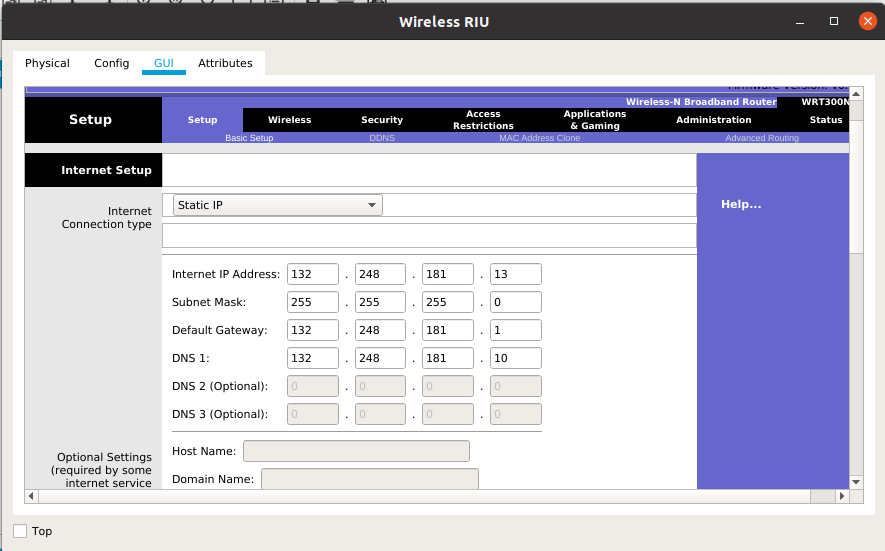
\includegraphics[scale=0.3]{imagenes/1}

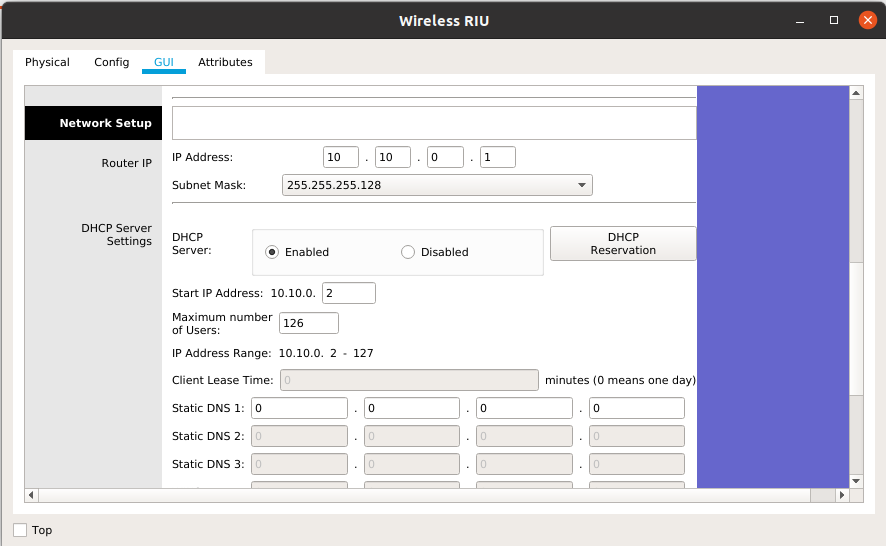
\includegraphics[scale=0.3]{imagenes/2}

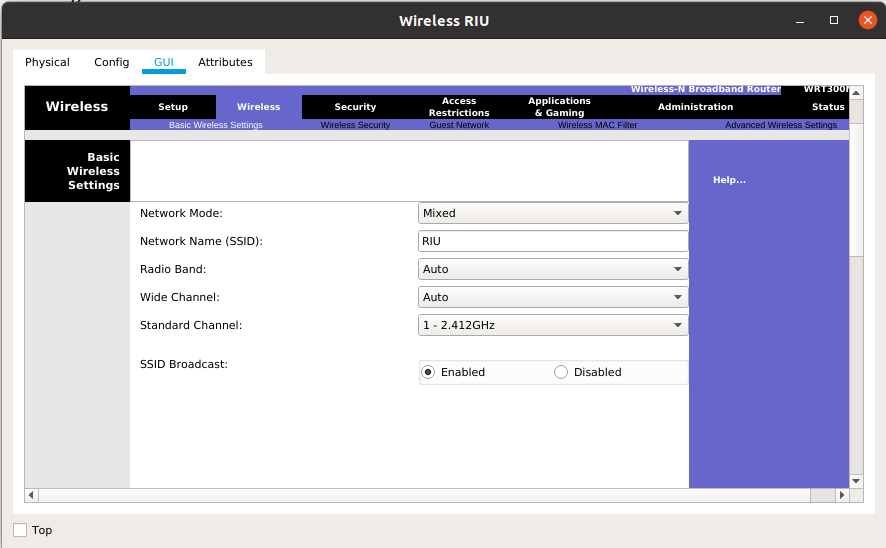
\includegraphics[scale=0.3]{imagenes/3}
\end{center}

Se agregó una Laptop con nombre VAIO para conectarse a la red inalámbrica de RIU. Para que se pueda conectar se debe apagar la computadora, quitar el FastEthernet, agregar el PT-LAPTOP-NM-1W y volver a encenderla.

\begin{center}
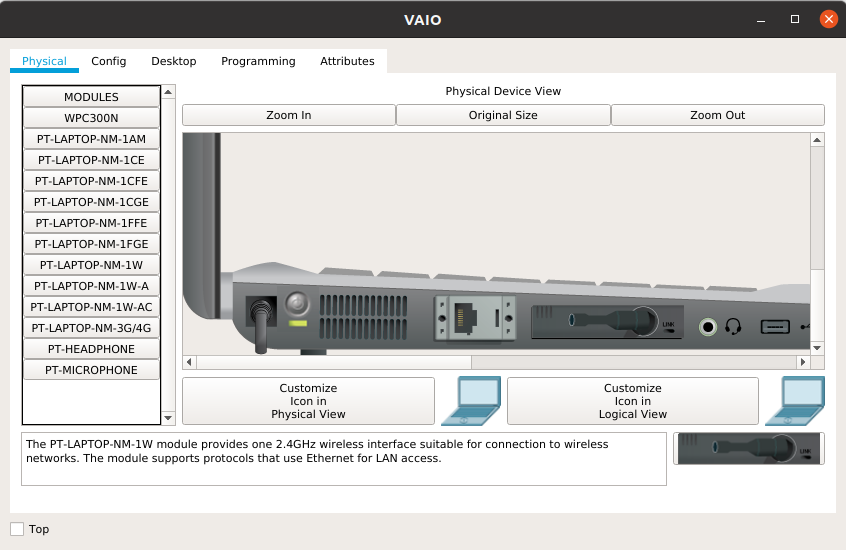
\includegraphics[scale=0.3]{imagenes/4}
\end{center}

Agregar un smartphone. Conectar la laptop y el smartphone a la red inalámbrica, colocando RIU en el SSID y asignándole una dirección IP mediante DHCP.

\begin{center}
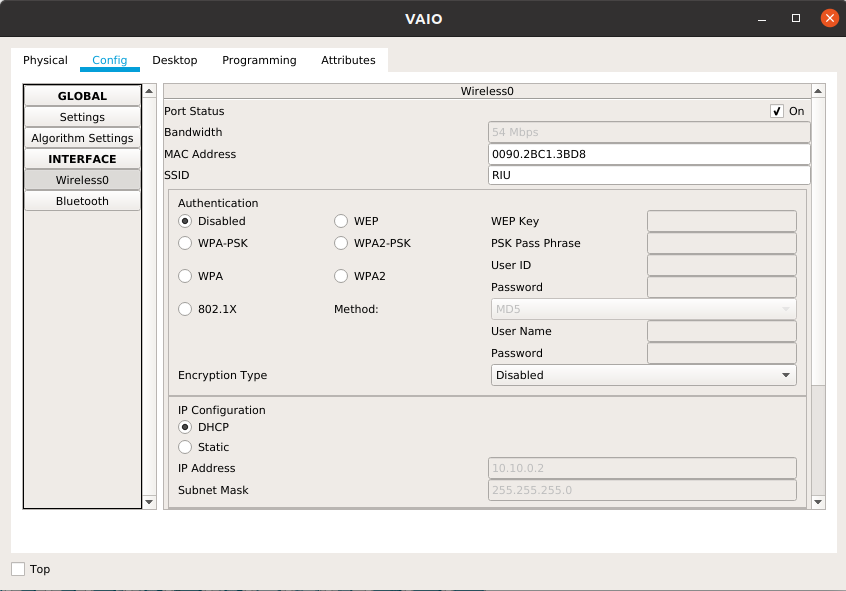
\includegraphics[scale=0.3]{imagenes/5}

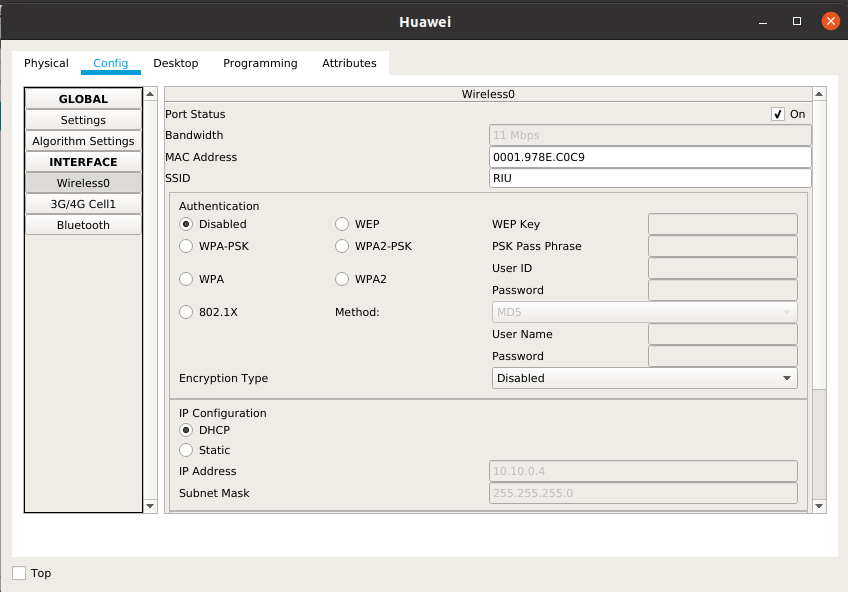
\includegraphics[scale=0.3]{imagenes/6}
\end{center}

El siguiente paso es configurar un servidor web con los parámetros que se muestran en la tabla.

\begin{center}
\begin{tabular}{|l|l|}
\hline
IP Address & 132.248.181.11 \\ \hline
Netmask & 255.255.255.0 \\ \hline
Gateway & 132.248.181.1 \\ \hline
DNS & 132.248.181.10 \\ \hline
URL & www.fciencias.unam.mx \\ \hline
\end{tabular}
\end{center}

\begin{center}
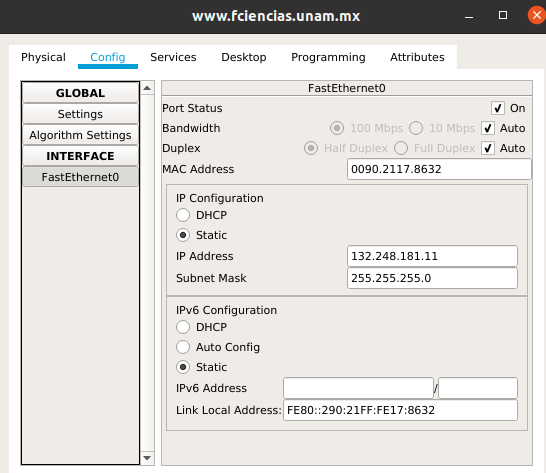
\includegraphics[scale=0.3]{imagenes/7}

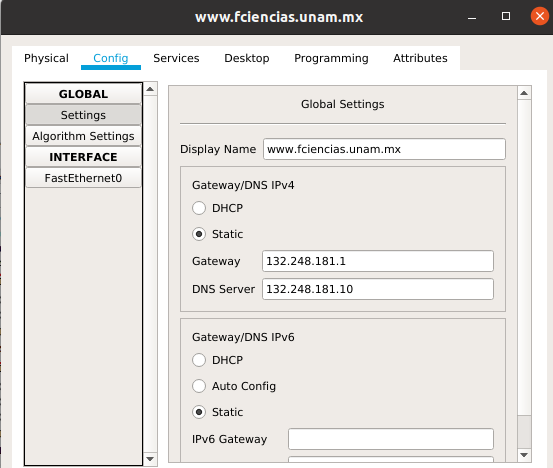
\includegraphics[scale=0.3]{imagenes/8}
\end{center}

En el index.html se coloca el nombre del alumno.

\begin{center}
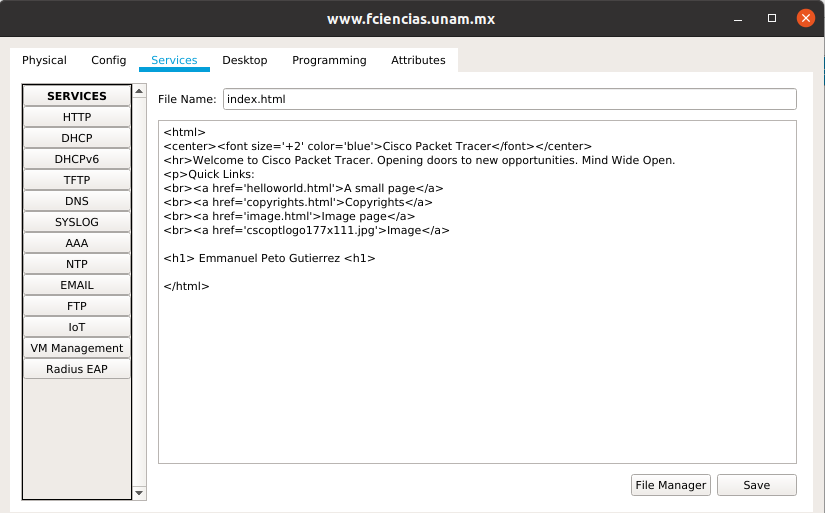
\includegraphics[scale=0.3]{imagenes/9}
\end{center}

Se configura un servidor DNS con los parámetros mostrados en la tabla. Se debe apagar el servicio HTTP y HTTPS.

\begin{center}
\begin{tabular}{|l|l|}
\hline
IP Address & 132.248.181.10 \\ \hline
Netmask & 255.255.255.0 \\ \hline
Gateway & 132.248.181.1 \\ \hline
\end{tabular}
\end{center}

\begin{center}
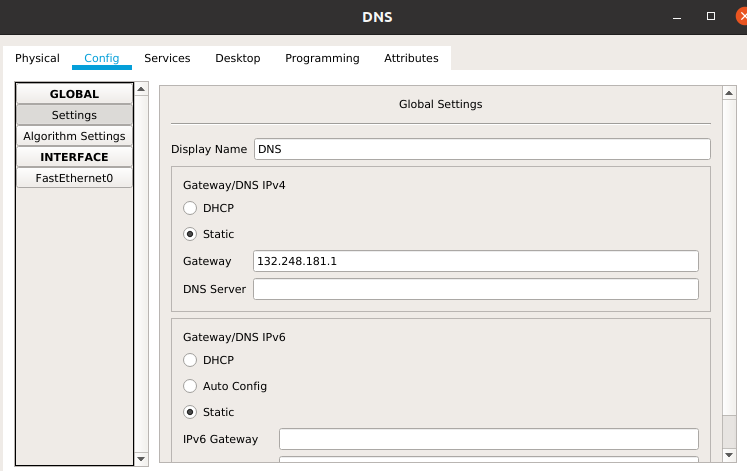
\includegraphics[scale=0.3]{imagenes/10}

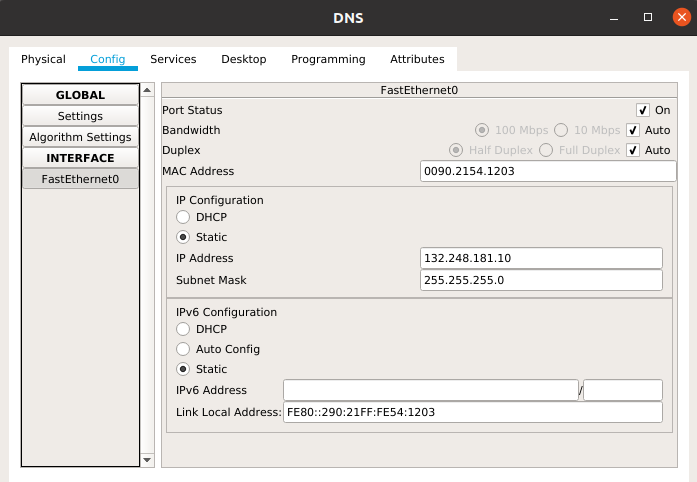
\includegraphics[scale=0.3]{imagenes/11}
\end{center}

Se enciende el servicio DNS y se agregan los registros mostrados en la tabla.

\begin{center}
\begin{tabular}{|l|l|l|}
\hline
\textbf{Name} & \textbf{Type} & \textbf{Detail} \\ \hline
ptolomeo.fciencias.unam.mx & A & 132.248.181.11 \\ \hline
www.fciencias.unam.mx & CNAME & ptolomeo.fciencias.unam.mx \\ \hline
\end{tabular}
\end{center}

\begin{center}
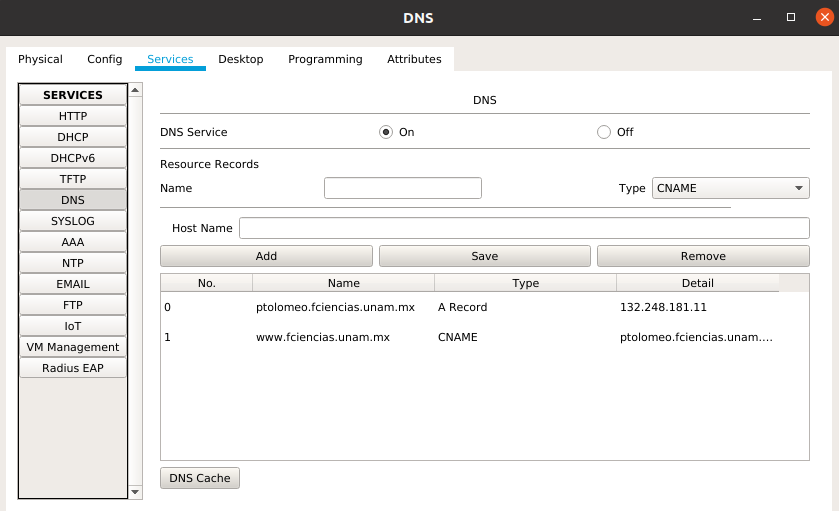
\includegraphics[scale=0.3]{imagenes/12}
\end{center}

Hasta el momento, la red debe estar como se muestra en la siguiente imagen.

\begin{center}
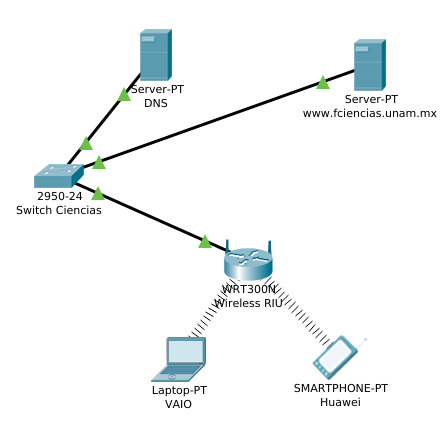
\includegraphics[scale=0.3]{imagenes/13}
\end{center}

Hay que probar que sí se puede acceder a la página \texttt{www.fciencias.unam.mx}. Para eso se abre el \textit{Web browser} en la laptop y se coloca la URL.

\begin{center}
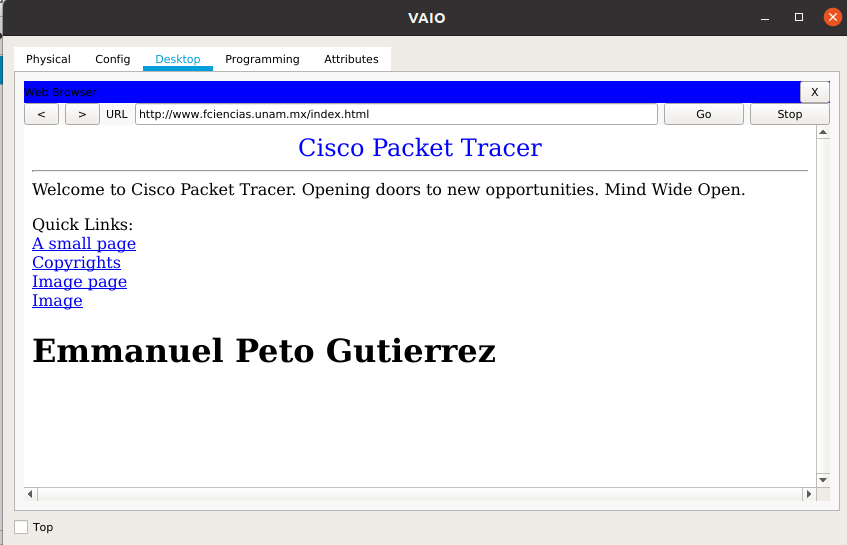
\includegraphics[scale=0.3]{imagenes/14}
\end{center}

Se abre un \textit{Command prompt} y se hace una consulta a \texttt{www.fciencias.unam.mx} mediante \texttt{nslookup} y se debe ver el nombre del servidor DNS.

\begin{center}
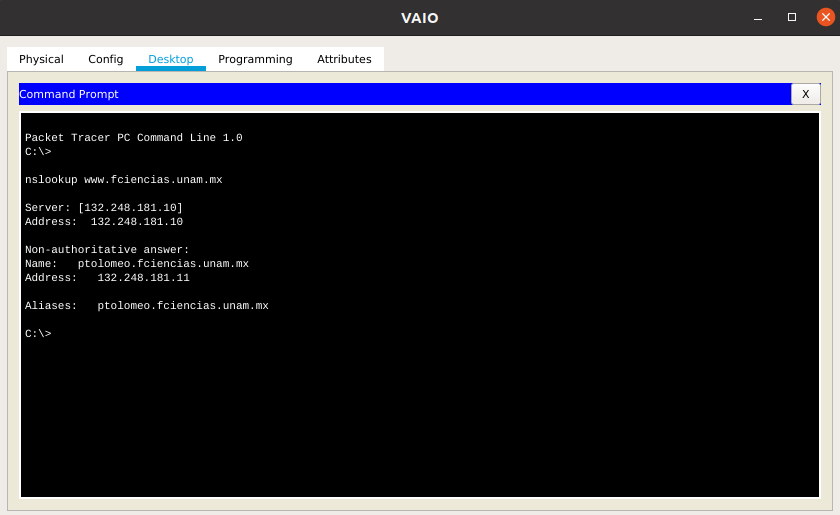
\includegraphics[scale=0.3]{imagenes/15}
\end{center}

Se configura un servidor DHCP para el laboratorio A. En las siguientes tablas se muestran las configuraciones.

\begin{center}
\begin{tabular}{|l|l|}
\hline
IP Address & 192.168.10.2 \\ \hline
Netmask & 255.255.255.0 \\ \hline
Gateway & 192.168.10.1 \\ \hline
DNS & 132.248.181.10 \\ \hline
\end{tabular}
\end{center}

\begin{center}
\begin{tabular}{|l|l|}
\hline
Default Gateway & 192.168.10.1 \\ \hline
DNS & 132.248.181.10 \\ \hline
Start IP Address & 192.168.10.4 \\ \hline
Netmask & 255.255.255.0 \\ \hline
Max. number of users & 120 \\ \hline
\end{tabular}
\end{center}

\begin{center}
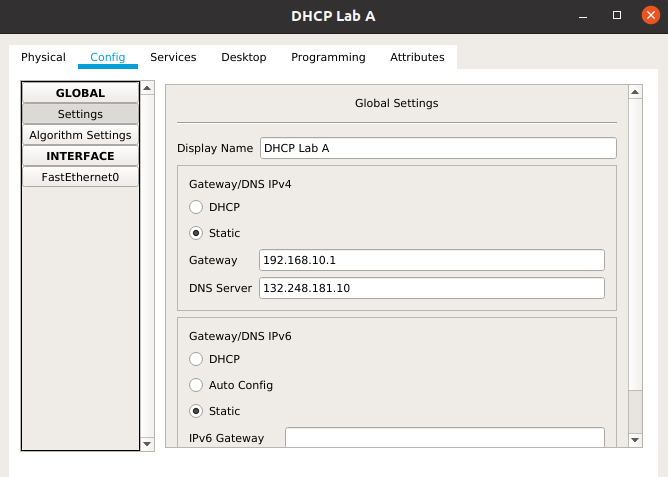
\includegraphics[scale=0.3]{imagenes/16}

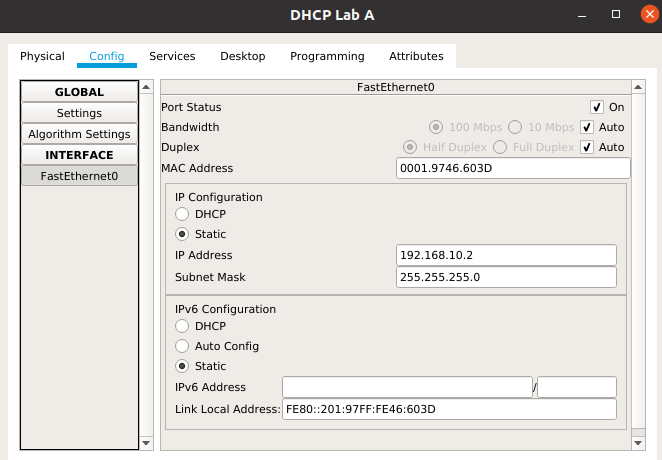
\includegraphics[scale=0.3]{imagenes/17}

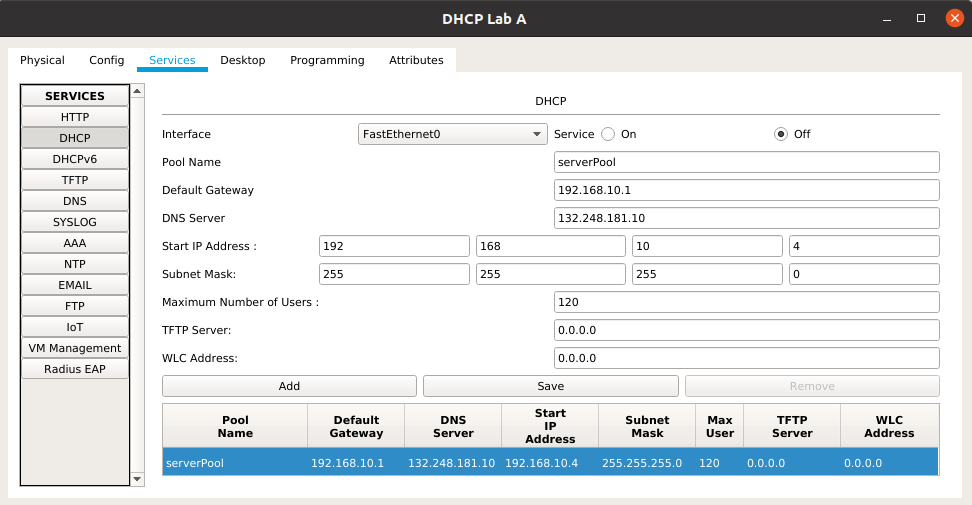
\includegraphics[scale=0.3]{imagenes/18}
\end{center}

Se agrega y se configura una impresora para el laboratorio A.

\begin{center}
\begin{tabular}{|l|l|}
\hline
IP Address & 192.168.10.3 \\ \hline
Netmask & 255.255.255.0 \\ \hline
Gateway & 192.168.10.1 \\ \hline
DNS & 132.248.181.10 \\ \hline
\end{tabular}
\end{center}

\begin{center}
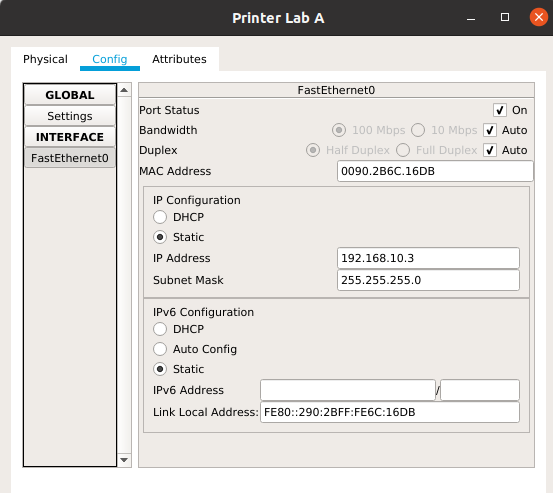
\includegraphics[scale=0.3]{imagenes/19}

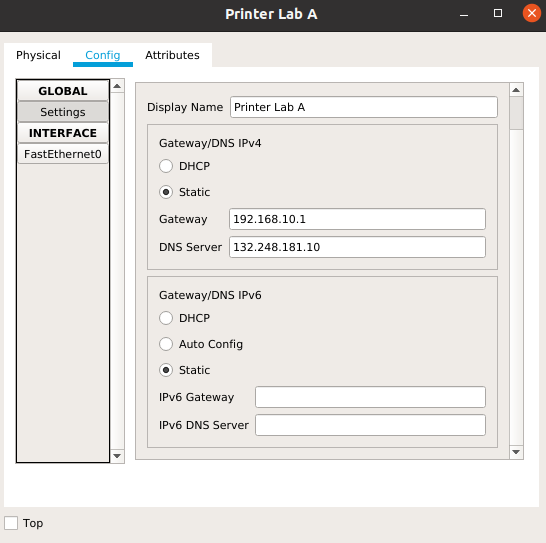
\includegraphics[scale=0.3]{imagenes/20}
\end{center}

Se agregan dos computadoras para el laboratorio A asignando sus direcciones IP de manera dinámica mediante el servidor DHCP.

Después se agrega un router y se conecta al switch del laboratorio A. Se debe configurar el NAT/PAT. En la interfaz física se agregan dos interfaces Fast Ethernet con NM-2FE2W.

\begin{center}
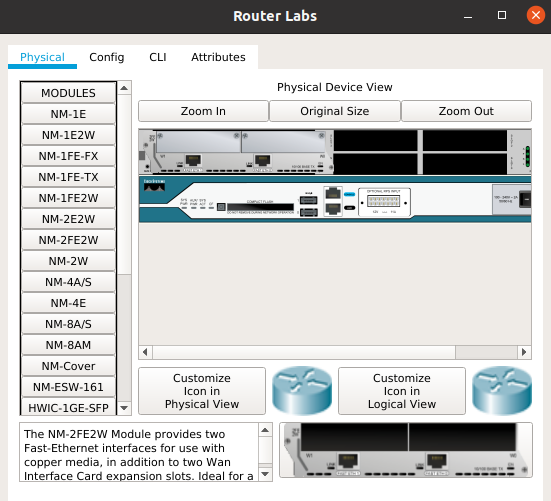
\includegraphics[scale=0.3]{imagenes/21}
\end{center}

El router se configura mediante la consola de comandos.

\begin{center}
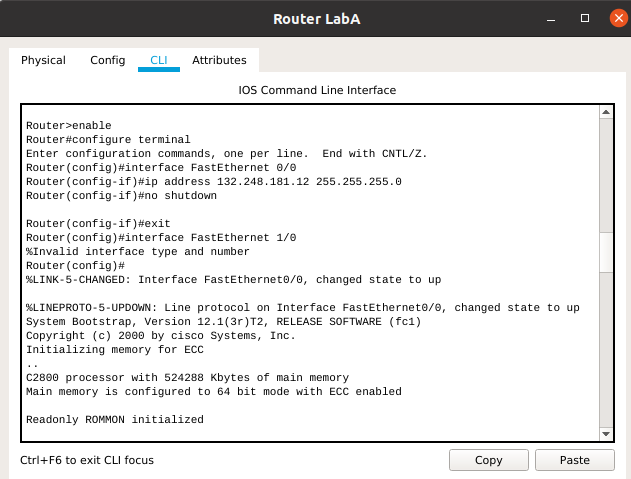
\includegraphics[scale=0.3]{imagenes/24}

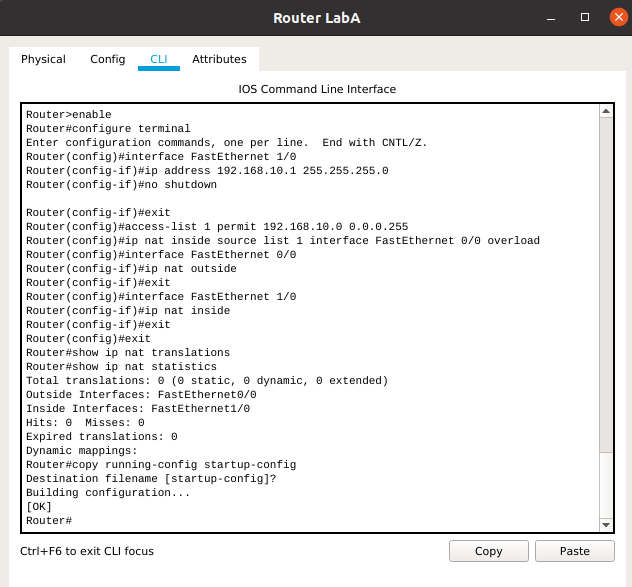
\includegraphics[scale=0.3]{imagenes/25}
\end{center}

Se puede comprobar la configuración ingresando a la URL \texttt{www.fciencias.unam.mx} desde una PC del laboratorio.

\begin{center}
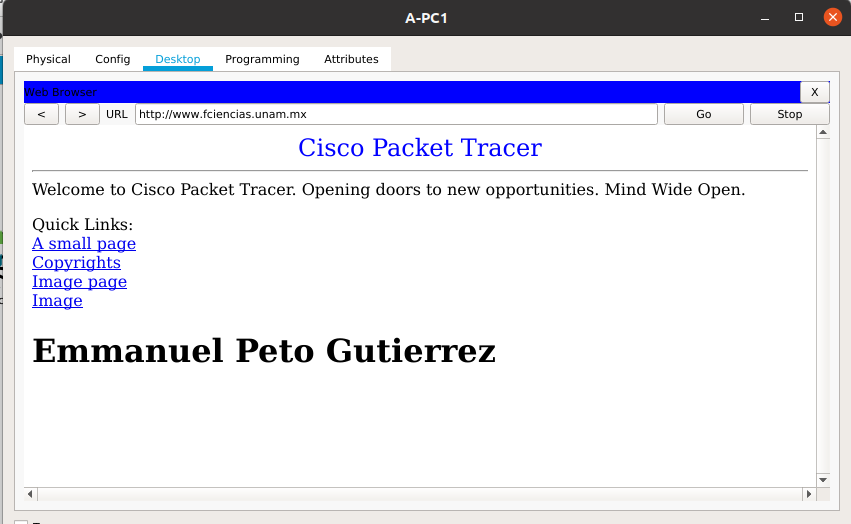
\includegraphics[scale=0.3]{imagenes/26}
\end{center}

Antes de agregar la red DGTIC hay que terminar de configurar el DNS de la Facultad de Ciencias. Para esto solo hay que agregar el DNS 132.247.70.2.

\begin{center}
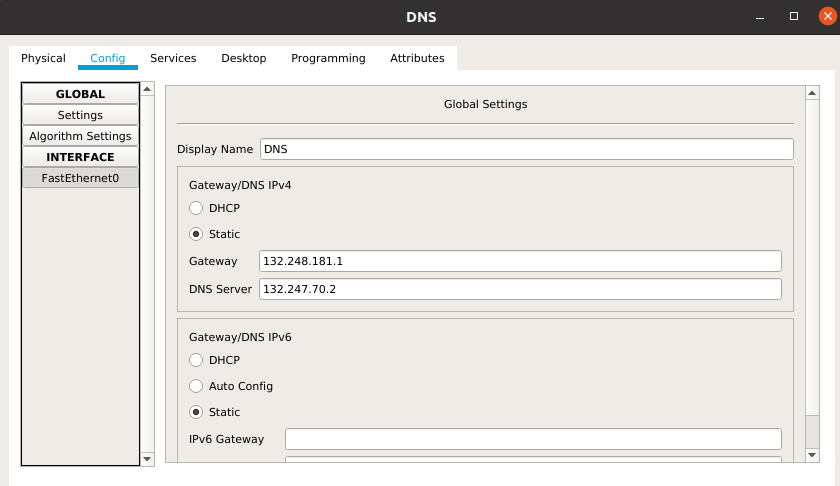
\includegraphics[scale=0.3]{imagenes/27}
\end{center}

\subsection{DGTIC}

En la red DGTIC se agregan dos PCs con las siguientes configuraciones.

\begin{center}
\begin{tabular}{|l|l|l|l|l|l|}
\hline
\textbf{Dispositivo} & \textbf{Nombre} & \textbf{Dir. IP} & \textbf{Máscara} & \textbf{Gateway} & \textbf{DNS} \\ \hline
PC-PT & PC1-DGTIC & 132.248.148.10 & 255.255.255.0 & 132.248.148.1 & 132.247.70.2 \\ \hline
PC-PT & PC2-DGTIC & 132.248.148.11 & 255.255.255.0 & 132.248.148.1 & 132.247.70.2 \\ \hline
\end{tabular}
\end{center}

\begin{center}
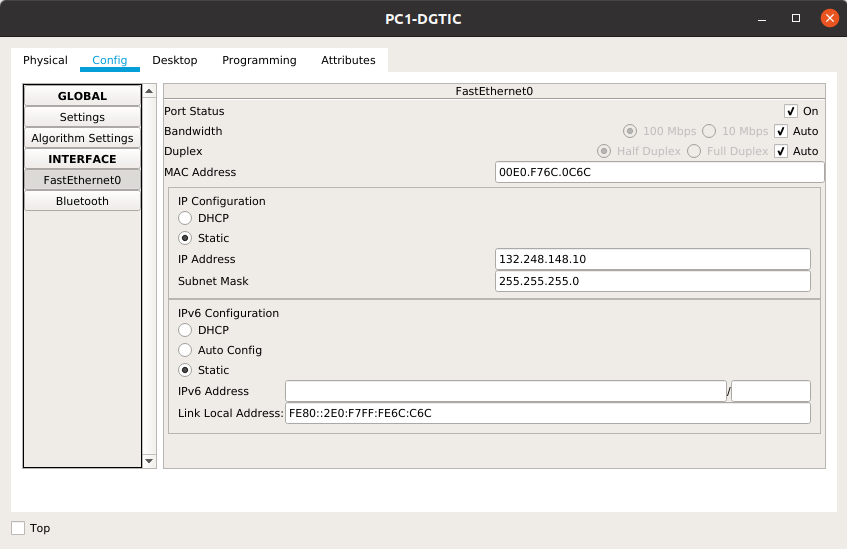
\includegraphics[scale=0.3]{imagenes/28}

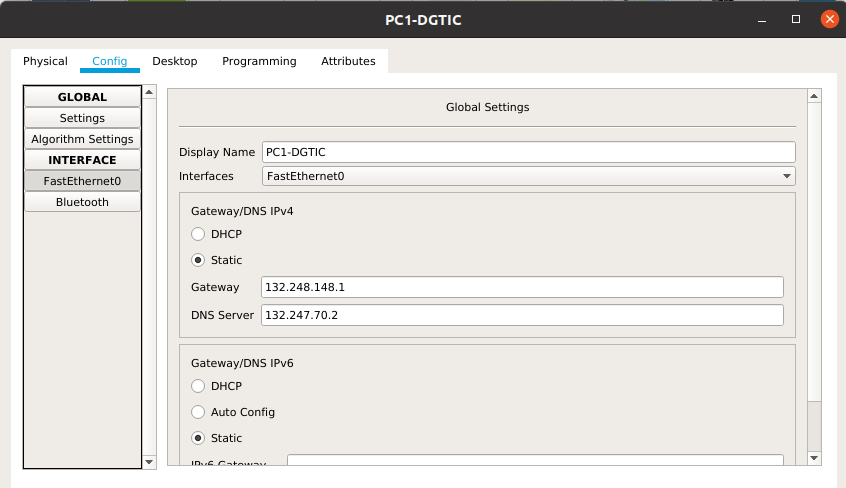
\includegraphics[scale=0.3]{imagenes/29}

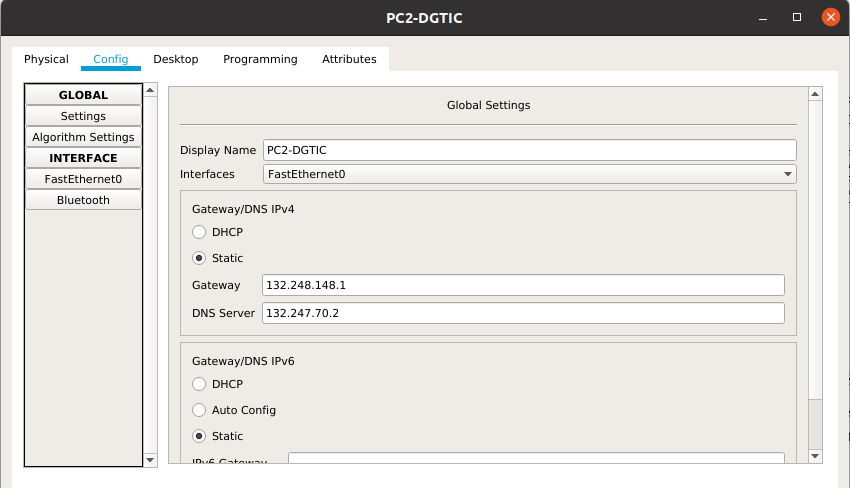
\includegraphics[scale=0.3]{imagenes/30}

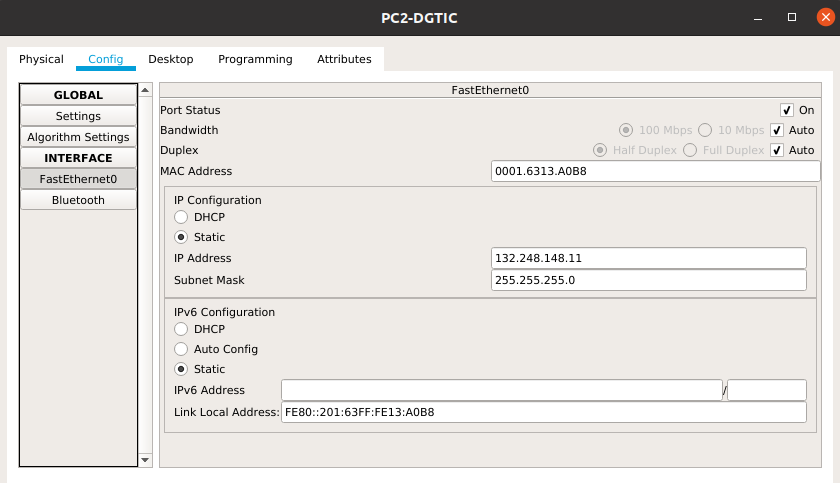
\includegraphics[scale=0.3]{imagenes/31}
\end{center}

En otra subred de DGTIC se configuran los servidores con los siguientes parámetros.

\begin{center}
\begin{tabular}{|l|l|l|l|l|}
\hline
\textbf{Nombre} & \textbf{Dir. IP} & \textbf{Máscara} & \textbf{Gateway} & \textbf{DNS} \\ \hline
ns1.unam.mx & 132.247.70.2 & 255.255.255.0 & 132.247.70.1 & \\ \hline
www.unam.mx & 132.247.70.3 & 255.255.255.0 & 132.247.70.1 & 132.247.70.2 \\ \hline
www.dgapa.unam.mx & 132.247.70.4 & 255.255.255.0 & 132.247.70.1 & 132.247.70.2 \\ \hline
\end{tabular}
\end{center}

\begin{center}
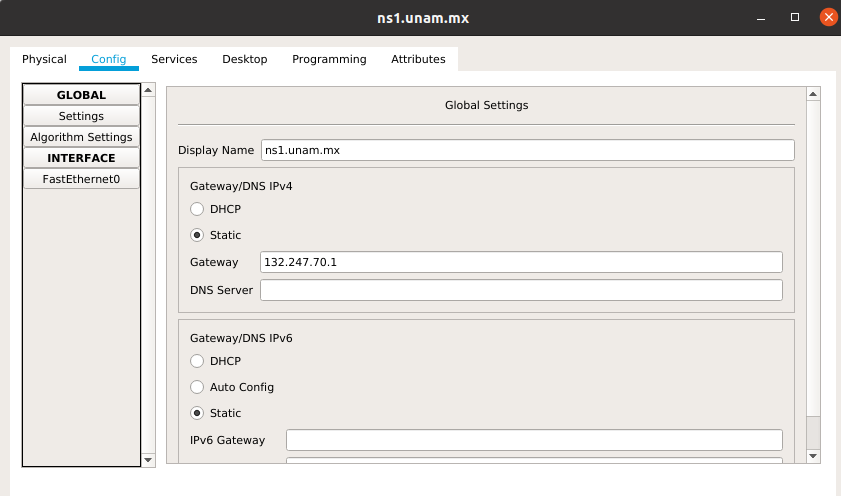
\includegraphics[scale=0.3]{imagenes/32}

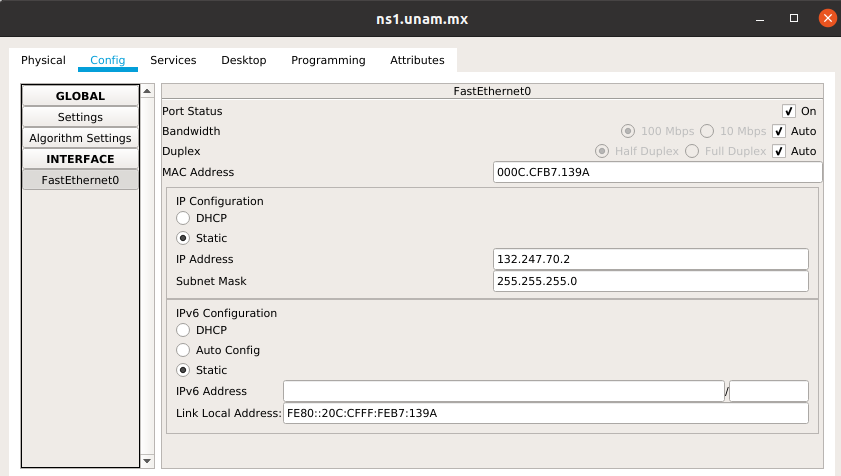
\includegraphics[scale=0.3]{imagenes/33}

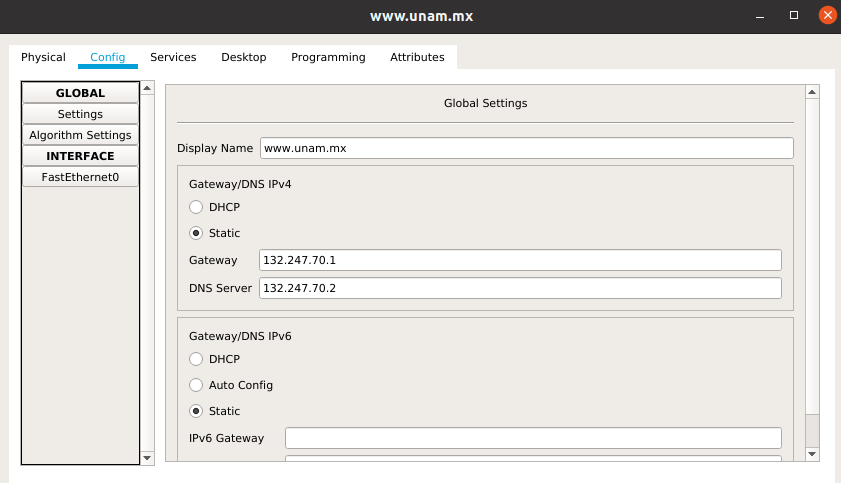
\includegraphics[scale=0.3]{imagenes/34}

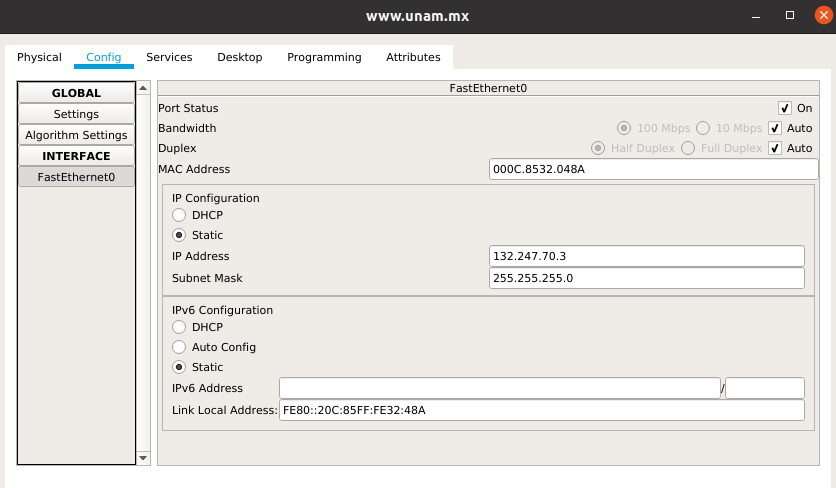
\includegraphics[scale=0.3]{imagenes/35}

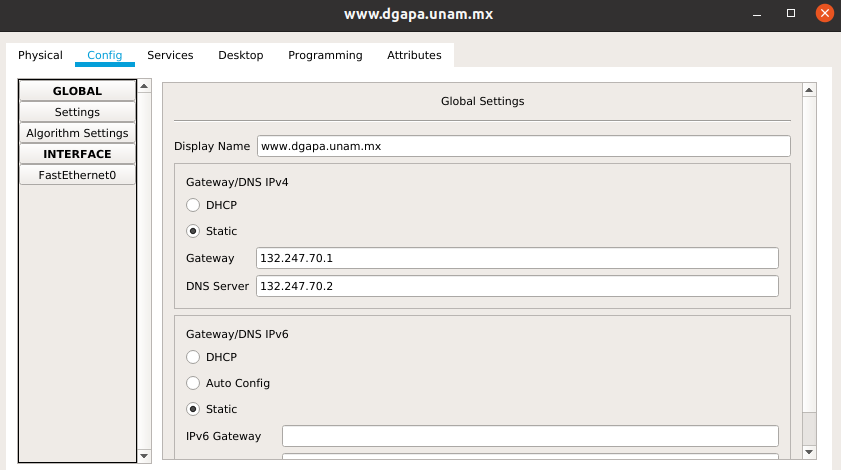
\includegraphics[scale=0.3]{imagenes/36}
\end{center}

En los servidores \texttt{www.unam.mx} y \texttt{www.dgapa.unam.mx} se modifica el archivo \texttt{index.html} colocando $<$h1$>$UNAM$<$/h1$>$ y $<$h1$>$DGAPA$<$/h1$>$ respectivamente.

Se agregan registros al servidor DNS de la Facultad de Ciencias como se muestra en las siguientes tablas.

\begin{center}
\begin{tabular}{|l|l|l|}
\hline
\textbf{Name} & \textbf{Type} & \textbf{Address} \\ \hline
ns1.unam.mx & A & 132.247.70.2 \\ \hline
nsfciencias.unam.mx & A & 132.248.181.10 \\ \hline
ptolomeo.fciencias.unam.mx & A & 132.248.181.11 \\ \hline
\end{tabular}
\end{center}

\begin{center}
\begin{tabular}{|l|l|l|}
\hline
\textbf{Name} & \textbf{Type} & \textbf{Host name} \\ \hline
www.fciencias.unam.mx & CNAME & ptolomeo.fciencias.unam.mx \\ \hline
\end{tabular}
\end{center}

\begin{center}
\begin{tabular}{|l|l|l|}
\hline
\textbf{Name} & \textbf{Type} & \textbf{Server name} \\ \hline
unam.mx & NS & ns1.unam.mx \\ \hline
\end{tabular}
\end{center}

\begin{center}
\begin{tabular}{|l|l|}
\hline
\textbf{Name} & fciencias.unam.mx \\ \hline
\textbf{Type} & SOA \\ \hline
\textbf{Primary Server Name} & nsfciencias.unam.mx \\ \hline
\textbf{Mail Box} & mail.fciencias.unam.mx \\ \hline
\textbf{Minimum TTL} & 9527 \\ \hline
\textbf{Refresh time} & 7200 \\ \hline
\textbf{Retry time} & 7200 \\ \hline
\textbf{Expiry time} & 86400 \\ \hline
\end{tabular}
\end{center}

\begin{center}
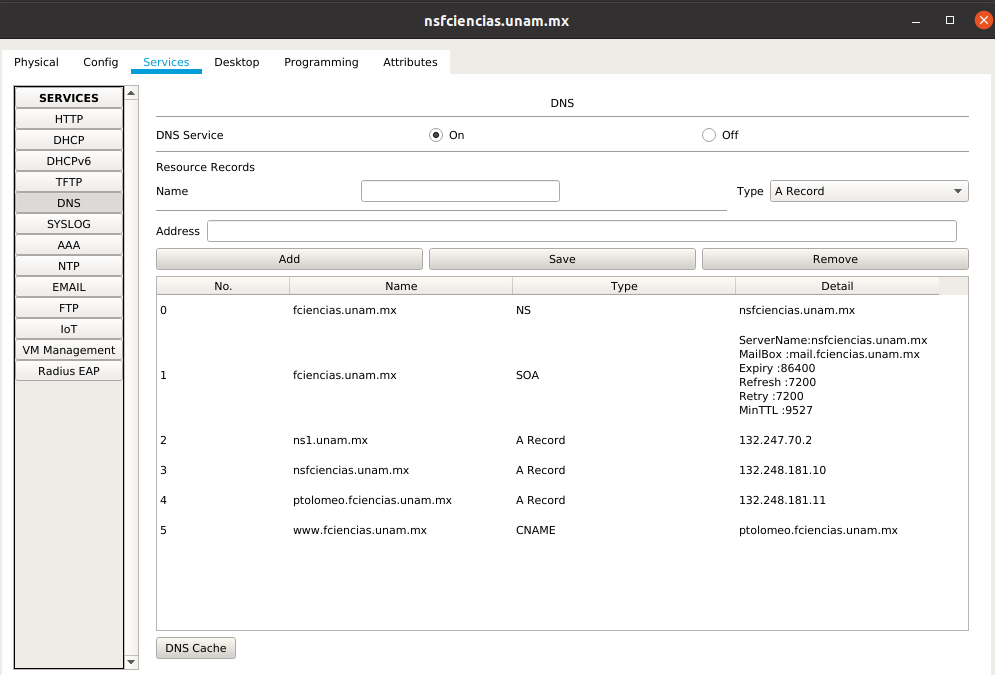
\includegraphics[scale=0.3]{imagenes/37}
\end{center}

En la red DGTIC también se agrega un servidor DNS y se configura de manera similar a como se configuró el de la Facultad de Ciencias.

\begin{center}
\begin{tabular}{|l|l|l|}
\hline
\textbf{Name} & \textbf{Type} & \textbf{Address} \\ \hline
ns1.unam.mx & A & 132.247.70.2 \\ \hline
nsfciencias.unam.mx & A & 132.248.181.10 \\ \hline
www.dgapa.unam.mx & A & 132.247.70.4 \\ \hline
www.unam.mx & A & 132.247.70.3 \\ \hline
\end{tabular}
\end{center}

\begin{center}
\begin{tabular}{|l|l|l|}
\hline
\textbf{Name} & \textbf{Type} & \textbf{Server name} \\ \hline
fciencias.unam.mx & NS & nsfciencias.unam.mx \\ \hline
\end{tabular}
\end{center}

\begin{center}
\begin{tabular}{|l|l|}
\hline
\textbf{Name} & unam.mx \\ \hline
\textbf{Type} & SOA \\ \hline
\textbf{Primary Server Name} & ns1.unam.mx \\ \hline
\textbf{Mail Box} & mail.unam.mx \\ \hline
\textbf{Minimum TTL} & 9527 \\ \hline
\textbf{Refresh time} & 7200 \\ \hline
\textbf{Retry time} & 7200 \\ \hline
\textbf{Expiry time} & 86400 \\ \hline
\end{tabular}
\end{center}

\begin{center}
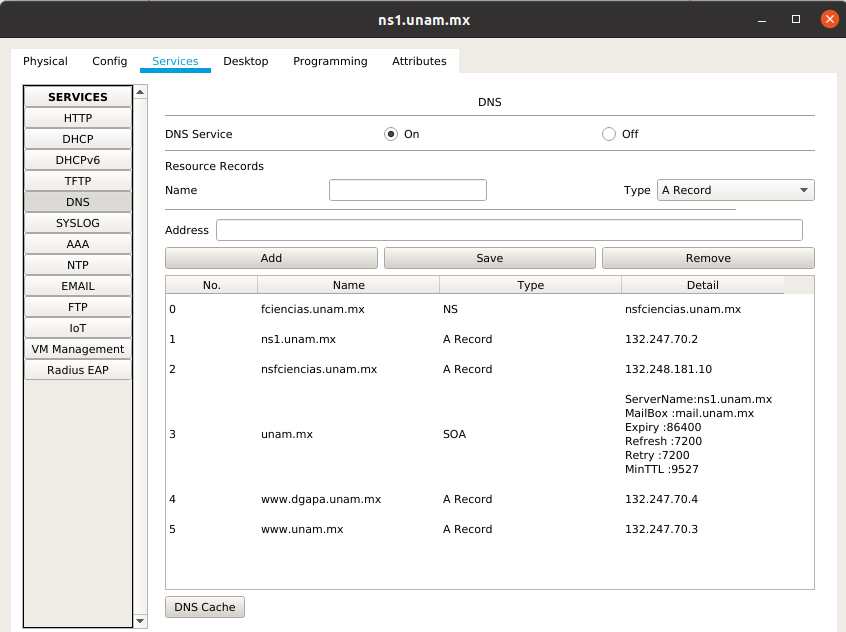
\includegraphics[scale=0.3]{imagenes/38}
\end{center}

Se configuran los hostname de los routers de la siguiente manera.

\begin{center}
\begin{tabular}{|l|l|}
\hline
\textbf{Dispositivo} & \textbf{Nombre} \\ \hline
Router ciencias & R-Ciencias \\ \hline
Router DGTIC & R-DGTIC \\ \hline
Router labs & R-LABS \\ \hline
SW-Core & SW-Core \\ \hline
\end{tabular}
\end{center}

\begin{center}
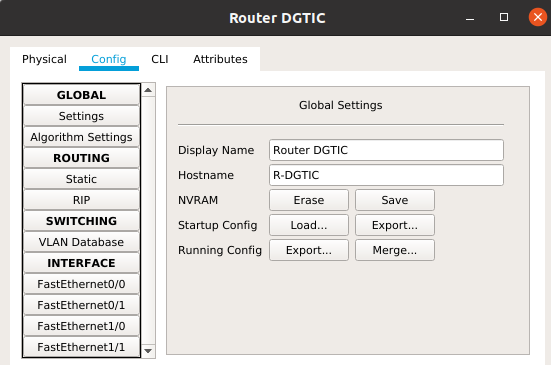
\includegraphics[scale=0.3]{imagenes/39}

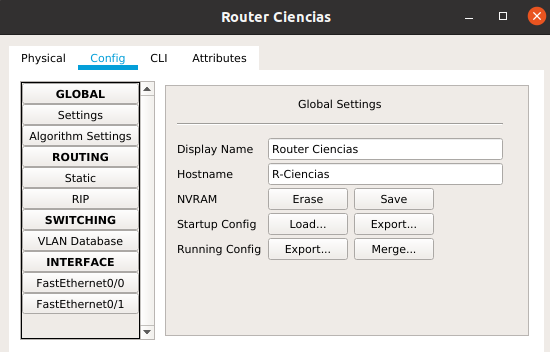
\includegraphics[scale=0.3]{imagenes/40}

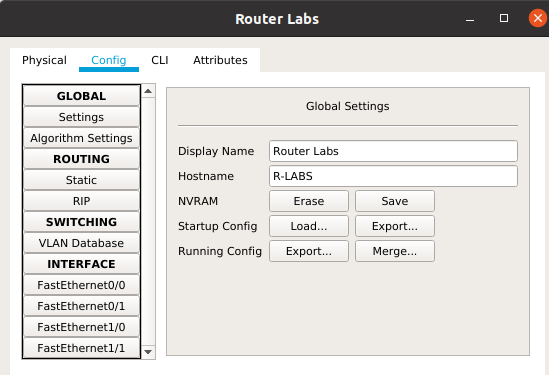
\includegraphics[scale=0.3]{imagenes/41}

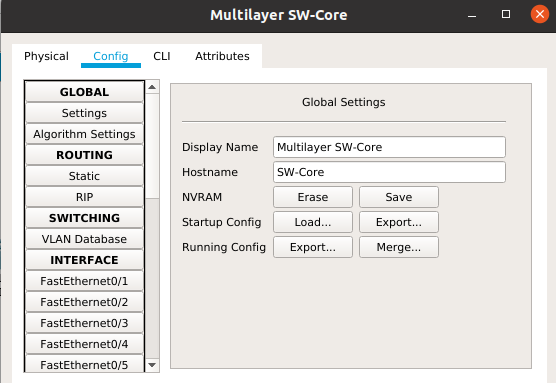
\includegraphics[scale=0.3]{imagenes/42}
\end{center}

Después se configuran las interfaces de red de los routers de Ciencias y DGTIC, y el switch de capa 3.

\begin{center}
Ciencias

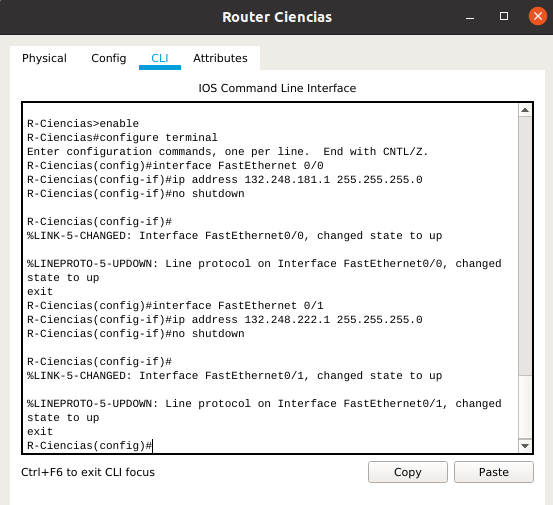
\includegraphics[scale=0.3]{imagenes/43}

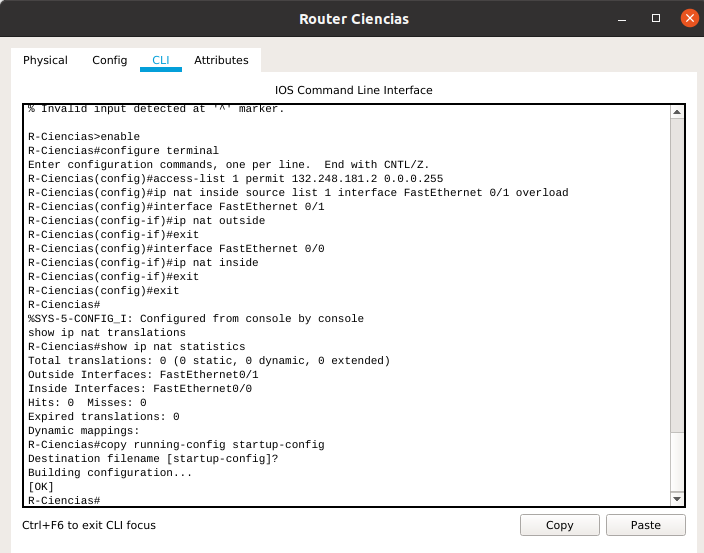
\includegraphics[scale=0.3]{imagenes/44}
\end{center}

\begin{center}
DGTIC

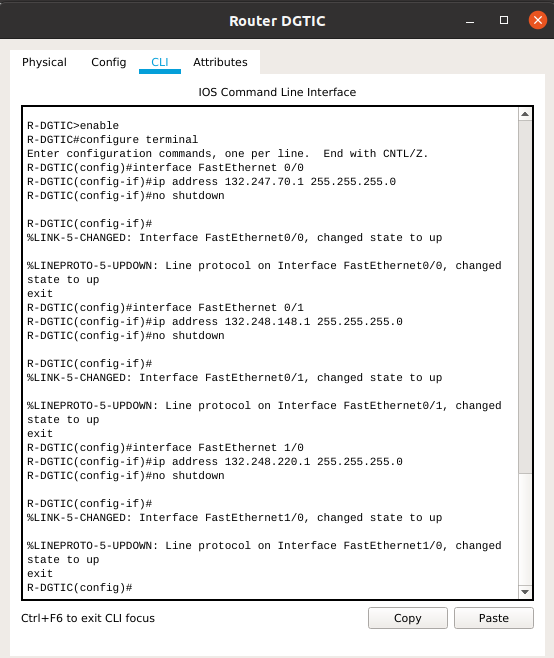
\includegraphics[scale=0.3]{imagenes/45}
\end{center}

\begin{center}
Switch

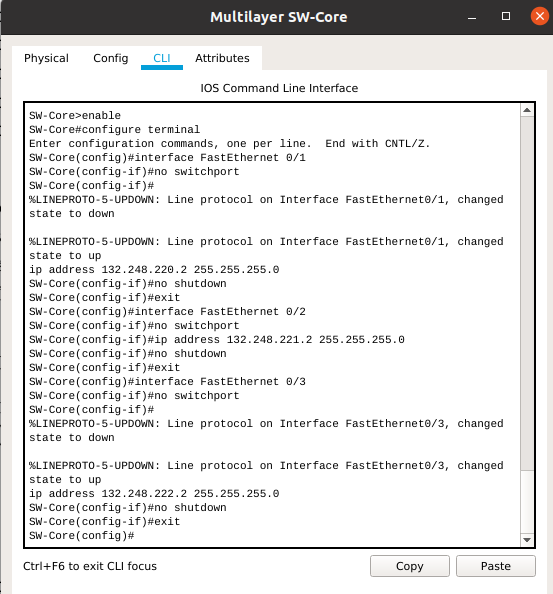
\includegraphics[scale=0.3]{imagenes/46}
\end{center}

Se puede comprobar que una PC de DGTIC puede acceder a las páginas \texttt{www.unam.mx} y \texttt{www.dgapa.unam.mx}.

\begin{center}
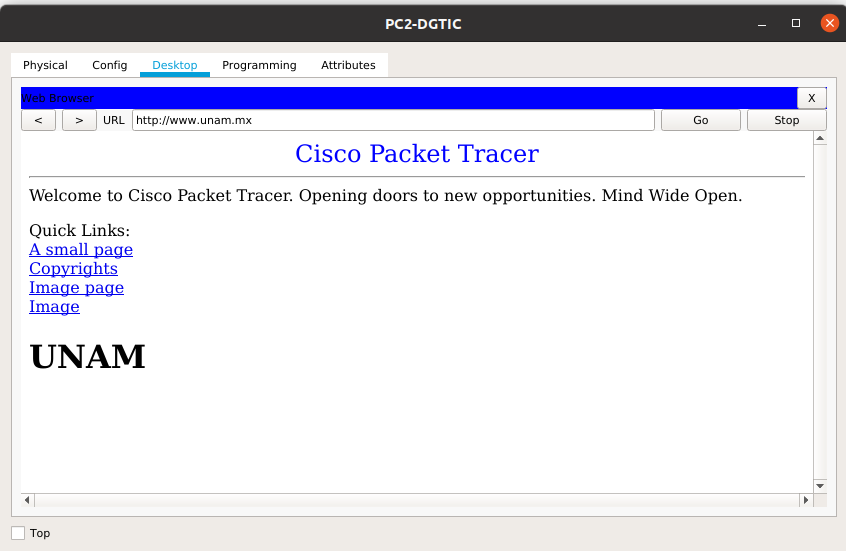
\includegraphics[scale=0.3]{imagenes/47}

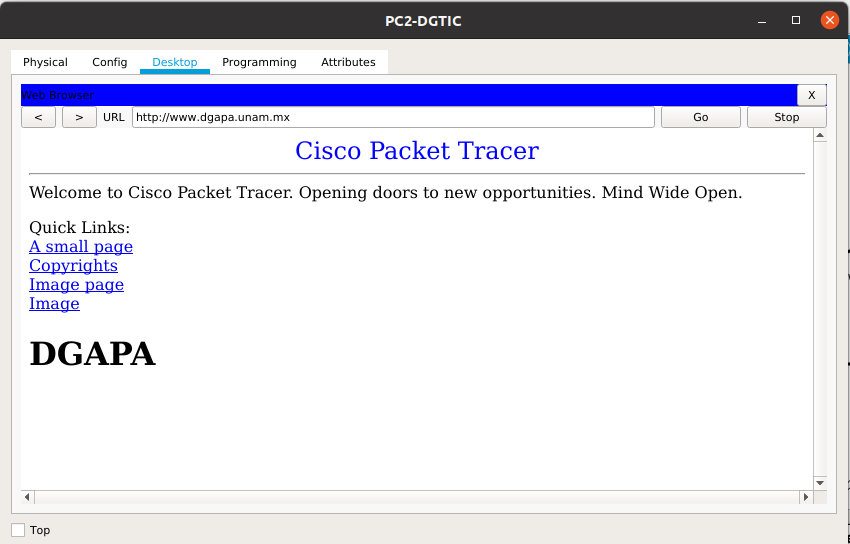
\includegraphics[scale=0.3]{imagenes/48}
\end{center}

A continuación se muestra la salida de los comandos \texttt{show ip route} y \texttt{show ip interface brief} en los routers de Labs, Ciencias y DGTIC.

\begin{center}
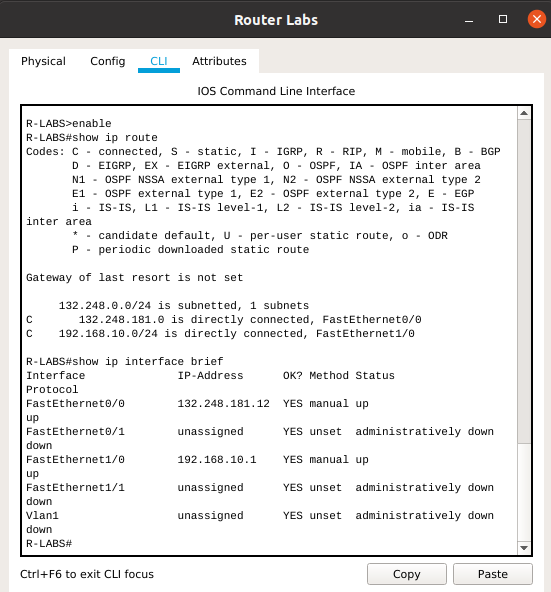
\includegraphics[scale=0.3]{imagenes/49}

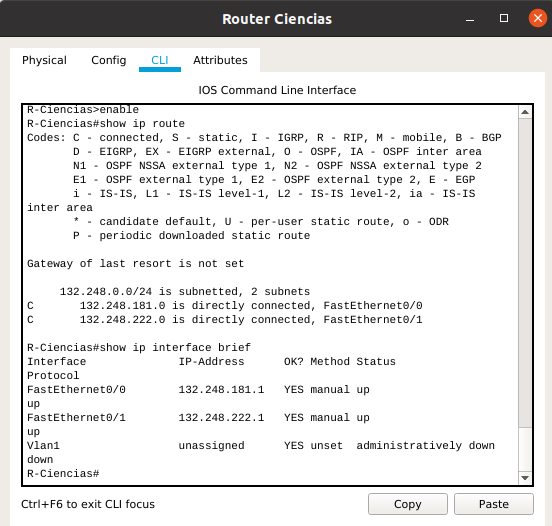
\includegraphics[scale=0.3]{imagenes/50}

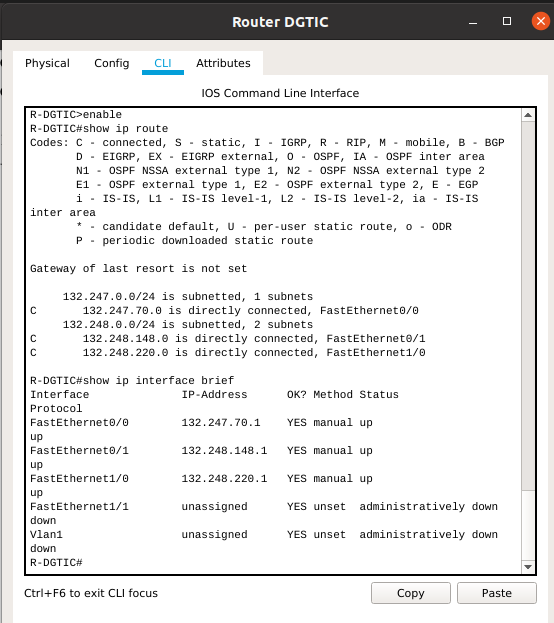
\includegraphics[scale=0.3]{imagenes/51}
\end{center}

Se comprueba que se puede acceder a \texttt{www.fciencias.unam.mx} desde la PC 2 del laboratorio A.

\begin{center}
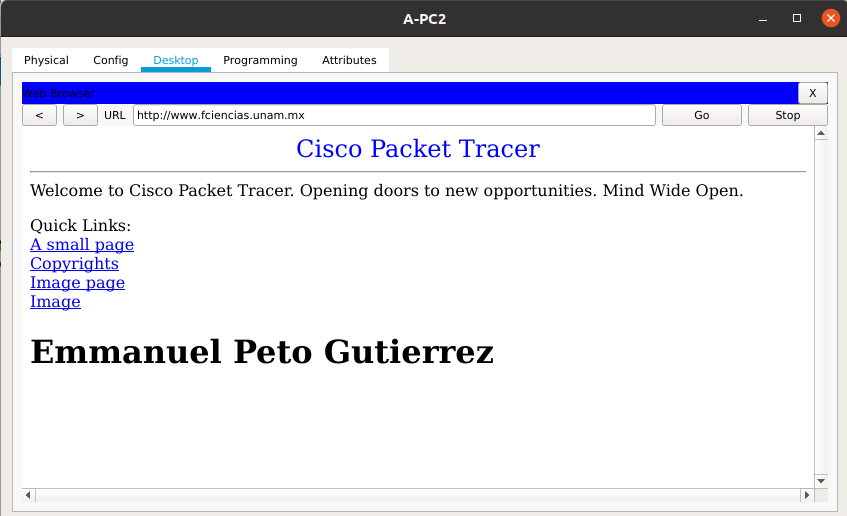
\includegraphics[scale=0.3]{imagenes/52}
\end{center}

Se muestra la memoria caché de los servidores DNS de Ciencias y DGTIC (que está vacía).

\begin{center}
\includegraphics[scale=0.3]{imagenes/53}

\includegraphics[scale=0.3]{imagenes/54}
\end{center}

La red final queda como en la siguiente figura.

\begin{center}
\includegraphics[scale=0.3]{imagenes/55}
\end{center}

\section{Cuestionario}

\begin{itemize}
\item[1.] \textbf{¿Qué direcciones IP le asignó el Router inalámbrico a cada host, a la Laptop y al smartphone, conectados a la red inalámbrica RIU?}

$\bullet$ Laptop: 10.10.0.3\\
$\bullet$ Smartphone: 10.10.0.2

\item[2.] \textbf{¿Qué direcciones IP le asignó el servidor DHCP a cada host de la red del Laboratorio
A?}

$\bullet$ A-PC1: 192.168.10.5\\
$\bullet$ A-PC2: 192.168.10.4

\item[3.] \textbf{Investigue el concepto de DHCP y explique.}

El significado de DHCP es \textit{Dynamic Host Configuration Protocol} y permite a los host obtener una dirección IP de manera automática en una red. También le permite obtener información adicional como la máscara de subred, la dirección del default gateway y la dirección de su servidor DNS local.

Para obtener la dirección IP de manera dinámica, se realiza una interacción entre el cliente (host) y el servidor DHCP que consta de 4 pasos.

$\bullet$ \textbf{Discovery:} el cliente realiza un broadcast para descubrir algún servidor DHCP en la red en la que se intenta conectar.\\
$\bullet$ \textbf{Offer:} cuando un servidor DHCP recibe el mensaje de descubrimiento realiza un broadcast con un mensaje de oferta, el cual contiene un ID y la información que le provee el servidor (IP, máscara, etc).\\
$\bullet$ \textbf{Request:} el cliente responde a algún servidor DHCP con un mensaje de solicitud.\\
$\bullet$ \textbf{Ack:} el servidor le responde al cliente con un mensaje de reconocimiento, confirmando los parámetros solicitados.

\item[4.] \textbf{Investigue los conceptos de NAT y PAT, y explique.}

NAT significa \textit{Network Address Translation} y se implementa en un router. Este protocolo utiliza una tabla NAT cuya utilidad es que los dispositivos con direcciones IP privadas puedan comunicarse con el mundo exterior.

La tabla NAT asocia un número de puerto con una dirección IP privada. Así, cada vez que un host envía un paquete fuera de la red local, el router cambia la dirección IP privada del host por su IP pública y le asocia un número de puerto antes de enviarlo fuera de esa red.

PAT significa \textit{Port Address Translation}. Traduce el puerto de una dirección externa al puerto de una dirección interna.

\item[5.] \textbf{¿Qué es la máscara de red o Netmask?}

La máscara de subred es una secuencia de 32 bits que sirve para identificar la parte de una dirección IP que pertenece a la subred. Si en una subred los primeros 24 bits determinan la dirección de la subred entonces en la máscara se tendrán los primeros 24 bits encendidos (en 1) y los últimos 8 apagados (en 0).

Para obtener la dirección de la subred a partir de cualquier IP de algún dispositivo se aplica la operación AND bit a bit entre la dirección IP y la máscara.

Por ejemplo, si se tiene la dirección IP de algún dispositivo en una subred (en binario):\\
11000000.10101000.00000001.00000100

y la máscara de subred es:\\
11111111.11111111.11111111.00000000

se obtiene la dirección de la subred realizando un AND entre la dirección IP del dispositivo y la máscara:\\
11000000.10101000.00000001.00000000

O en decimal, con la dirección IP del dispositivo 192.168.1.4 y la máscara 255.255.255.0 se obtiene la dirección de la subred 192.168.1.0.

\item[6.] \textbf{¿Qué es la Puerta de Enlace predeterminada o Default Gateway?}

Es el primer router por el que pasa un paquete que sale de una red. Dicho de otra forma, es la puerta de salida de los dispositivos de una red que se comunican con el mundo exterior.

\item[7.] \textbf{¿Qué es el SSID en una red inalámbrica?}

El significado de SSID es \textit{Service Set Identifier}. Es el nombre asociado a un router inalámbrico y es el que se ve cuando un dispositivo busca las redes disponibles. 

\item[8.] \textbf{¿Cuáles son las funciones de un router en una red de computadoras?}

Algunas de las funciones de un router son las siguientes:

\begin{itemize}
\item Reenvían los paquetes de un router a otro, hasta que llegan a su destino final. Para esto usa una tabla de reenvío (\textit{forwarding table}).
\item Implementar protocolos NAT/PAT para comunicar una red privada con una pública.
\item Encolar paquetes recibidos para después procesarlos y reenviarlos.
\item Determinar la ruta que debe tomar un paquete para llegar a su destino.
\end{itemize}

\item[9.] \textbf{¿Qué son los protocolos de ruteo?}

Son algoritmos para calcular la ruta que debe seguir un paquete en una red para llegar a su destino. Los protocolos se implementan en los routers. Los algoritmos se usan para llenar las tablas de reenvío de los routers en el Internet.

\item[10.] \textbf{¿Qué es una ruta estática en un router?}

En un algoritmo estático de ruteo, las rutas cambian lentamente a lo largo del tiempo, por ejemplo, cuando se edita manualmente la tabla de reenvío de un router.

\item[11.] \textbf{Indique para que se usan los registros A, NS, CNAME y SOA en un servidor DNS.}

Los registros son tuplas de la forma (Name, Type, Value, TTL).

\begin{itemize}
\item Tipo A: Para este tipo, \textit{Name} es el nombre del host y \textit{Value} es la dirección IP para el nombre del host. Así que el tipo A cumple con la función principal de un DNS: proveer un mapeo de un hostname y una dirección IP. Por ejemplo, (relay1.bar.foo.com, 145.37.93.126, A).

\item Tipo NS: El \textit{Name} es un dominio y \textit{Value} es el hostname de un servidor DNS autoritativo que conoce cómo obtener la IP de ese dominio. Ejemplo, (foo.com, dns.foo.com, NS).

\item Tipo CNAME: \textit{Name} es un alias y \textit{Value} es el nombre canónico del host. Ejemplo, (foo.com, relay1.bar.foo.com, CNAME).

\item Tipo SOA: Es la autoridad de zona. Muestra características básicas del dominio y de la zona en la que se encuentra.
\end{itemize}

\end{itemize}

\end{document}

